\documentclass[a0]{sciposter}
\usepackage{multicol}
\usepackage{url}
\usepackage{graphicx}


\title{Webinterpret @ WMT2018\\Parallel Corpus Filtering Task}
\author{Marina Fomicheva and Jes\'{u}s Gonz\'{a}lez-Rubio}
\institute{AT Language Solutions, Webinterpret}
\email{\{mari.fomicheva, jesus.g.rubio\}@gmail.com}

\conference{{\bf WMT18}, Third conference on Machine translation (@ EMNLP-2018)}


% FIXME: update if necessary AT language solutions logo
\renewcommand\printleftlogo
  {\vspace*{10em}\hspace*{8em}\resizebox{10em}{!}{
\includegraphics{assets/logoAT.jpg}}
  }

\renewcommand\printrightlogo
  {\vspace*{8em}\hspace*{-10em}\resizebox{20em}{!}{
\includegraphics{assets/logoWI.png}}
  }


\begin{document}

\maketitle

\begin{multicols*}{2}

% FIXME: should we have an abstract?
%\begin{abstract}
%We describe the participation of Webinterpret in the shared task on parallel corpus filtering at WMT 2018: the main characteristics of our approach and the reported results.
%\end{abstract}


\section*{\Large Task Description and Proposed Approach}

\subsection*{Task Description:}
\begin{itemize}
  \item {\bf Goal:} from a noisy corpus, extract the best subset of sentence pairs for training
  \item {\bf Input:} noisy $1$-billion-word German--English corpus part of the Paracrawl project\footnote{\url{https://paracrawl.eu/}}
  \item {\bf Output:} a $100$-million-words and a $10$-million-words subsets of sentence pairs
  \item {\bf Evaluation criteria:} quality of translation systems trained on the selected data
  \begin{itemize}
    \item Statistical and Neural systems
    \item Two test sets: official WMT 2018 news translation test and a second undisclosed one
    \item BLEU metric
  \end{itemize}
\end{itemize}

\subsection*{Proposed Approach:}
\begin{itemize}
  \item Corpus filtering as a QE task
  \item {\bf Goal:} estimate to what extent a pair of sentences are translations of each other
  \item {\bf Approach:} given a pair of sentences $(\mathbf{s}, \mathbf{t})$
  \begin{enumerate}
    \item Compute features indicating to what extent the sentences correspond to each other
    \item Train a classification model on those features
    \item Select sentences with higher score according to the trained model
  \end{enumerate}
\end{itemize}


\section*{\Large Features}
\subsection*{Adequacy:} 
\begin{itemize}
  \item \textit{Average max lexical probability (2 f.)}: average maximum probability of word-to-word translation. Both source-to-target and target-to-source directions, e.g.  source-to-target:
  $$ \frac{1}{n}\sum_1^n\max_{j=0}^m P(t_i\mid s_j) $$
  where $\mathbf{s}=s_1\ldots s_m$, $\mathbf{t}=t_1\ldots t_n$, and $s_0$ indicates the \textit{NULL} word
  \item \textit{Cross-entropy (2 f.)}: ``distance'' between the sentences according to a bag-of-words model. Both source and target sentences, e.g. for source:
  $$\sum_{s_j\in\mathbf{s}}C_{\mathbf{s}}(s_j)\cdot\mathrm{log}\left(\frac{1}{C_{\mathbf{s}<\mathbf{t}}(s_j)}\right)$$
  where $C_{\mathbf{s}}(s_j)$ is count of word $s_j$ in $\mathbf{s}$, and $C_{\mathbf{s}<\mathbf{t}}(s_j)=\sum_{t_i\in\mathbf{t}}C_{\mathbf{t}}(t_i)P(s_j\mid t_i)$ is the count of $s_j$ estimated from $\mathbf{t}$ via a probabilistic lexicon 
\end{itemize}

\subsection*{Fluency:} 
\begin{itemize}
  \item \textit{Language model score (2 f.)}: log-probability of the source and target sentences
  \item \textit{Perplexity (2 f.)}: for both source and target sentences
\end{itemize}

\subsection*{Shape:}
\begin{itemize}
  \item \textit{Jaccard index (4 f.)}: similarity and diversity of sets of tokens in $\mathbf{s}$ and $\mathbf{t}$, applied to words, numbers, alphanumeric and punctuation tokens
  $$ \frac{\mid \mathcal{S}\cap \mathcal{T}\mid}{\mid \mathcal{S}\cup \mathcal{T}\mid}$$
  where $\mathcal{S}$ and $\mathcal{T}$ are sets of source/target tokens respectively
  \item \textit{Counts (8 f.)}: of words, numbers, alphanumeric and punctuation tokens in $\mathbf{s}$ and $\mathbf{t}$
  \item \textit{Counts difference (16 f.)}: ratio in both directions, absolute difference, and normalized absolute difference for the counts of words, numbers, alphanumeric and punctuation tokens
  \item \textit{Specific punctuation (12 f.)} absolute difference and normalized difference for counts of dots, commas, colons, semicolons, exclamation and question marks
\end{itemize}

~\newline
All features were computed from models trained on the News Commentary V13 parallel corpus as provided for the News translation task
\begin{itemize}
  \item \textit{Probabilistic lexicons:} sub-product of Moses training on its default configuration
  \item \textit{Language models:} $5$-gram models estimated with Kenlm
\end{itemize}


\section*{\Large Training Regime}
\subsection*{Initial consideration} 
how to obtain suitable examples to train the classification model?
\begin{itemize}
  \item \textit{Positive:} easy to obtain, e.g. sentences in a clean corpus such News Commentary V13
  \item \textit{Negative:} no readily available -there exist no collection of ``wrong'' sentence pairs- but they can be generated on-demand
\end{itemize}

\subsection*{Generation of negative examples}
\begin{itemize}
  \item Negative examples are ``perturbed'' version of positive sentence pairs
  \item We consider three different perturbation operations:
  \begin{itemize}
  \item \textit{Swap:} exchange source and target sentences
  \item \textit{Copy:} use same string in source and target
  \item \textit{Randomization:} replace one sentence in the pair by a random sentence in the corpus
  \end{itemize}
  \item Operations only mess with the correct correspondence between sentences
  \begin{itemize}
    \item Aim at identifying correctly aligned sentence pairs
    \item Alternative: estimate how valuable the pair is for training
    \begin{itemize}
      \item Not considered in this work, left for future developments
    \end{itemize}
  \end{itemize}
\end{itemize}

~\newline
Training examples were extracted from the News Commentary V13 parallel corpus
\begin{itemize}
  \item About $600$k training examples evenly distributed between positive and negative
  \item Negative examples were evenly distributed among the three perturbation operations
\end{itemize}


\section*{\Large Classification Model}
After initial tests, we choose Gradient Boosting\footnote{\url{https://en.wikipedia.org/wiki/Gradient_boosting}} as the classifier for our final submission
\begin{itemize}
  \item Model in the form of an ensemble of weak classifiers, typically decision trees
  \item Iterative construction of the final model
  \item Allow for the optimization of arbitrary differentiable loss functions
\end{itemize}

We use the implementation of gradient boosting from the scikit-learn library\footnote{\url{http://scikit-learn.org/stable/index.html}}
\begin{itemize}
  \item Prediction applied form each sentence pair in the noisy Paracrawl corpus
  \item Probability of the positive class submitted to the task
\end{itemize}


\section*{\Large Results}

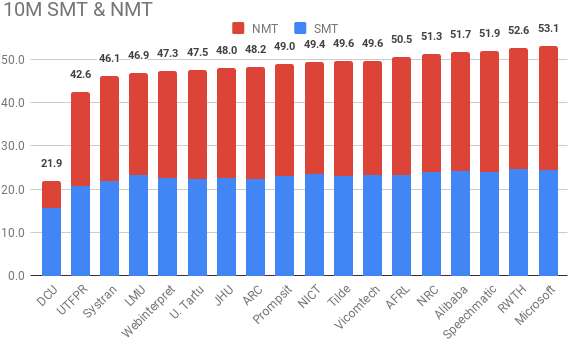
\includegraphics[width=\columnwidth]{assets/10M_crop.png}

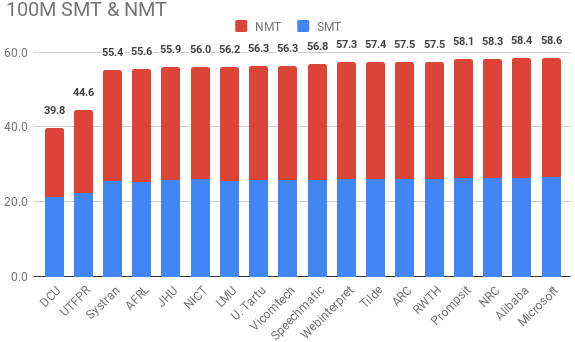
\includegraphics[width=\columnwidth]{assets/100M_crop.png}



\end{multicols*}

\end{document}